\SourcePage{678}{683}
\section{Double-logarithmic asymptotic form of the electron--muon scattering amplitude}

As an example of a different kind, consider the scattering of an electron by a negative muon, restricting the discussion to exact backward scattering, i.e. to the angle $\theta=\pi$ (\emph{V.~G.~Gorshkov, B.~N.~Gribov, L.~N.~Lipatov, G.~V.~Frolov}, 1967). This process is the simplest one in two respects. First, since the two particles are not identical, exchange diagrams are absent. Second, emission of soft photons is strongly suppressed in backward scattering, so no infrared divergence arises. Indeed, according to (98.8), the cross-section for soft-photon emission is
\begin{equation}
d\sigma=\alpha\left[\left(
\frac{\mathbf v'_e}{1-\mathbf v'_e\mathbf n}
+\frac{\mathbf v'_\mu}{1-\mathbf v'_\mu\mathbf n}
-\frac{\mathbf v_e}{1-\mathbf v_e\mathbf n}
-\frac{\mathbf v_\mu}{1-\mathbf v_\mu\mathbf n}
\right)\mathbf n\right]^2
\frac{d\omega\,do_{\mathbf n}}{4\pi^2\omega}\,d\sigma_{\text{el}},
\tag{137.1}
\end{equation}
where $\mathbf v_e$, $\mathbf v_\mu$ and $\mathbf v'_e$, $\mathbf v'_\mu$ are the particle velocities before and after the collision. In the ultrarelativistic case, however, equal momenta imply equal velocities, and to this accuracy, in the centre-of-mass

\SourcePage{679}{684}
system for backward scattering, $\mathbf v_e=-\mathbf v_\mu=-\mathbf v'_e=\mathbf v'_\mu$. Expression (137.1) therefore vanishes.

If the scattering process under consideration belongs to the $s$ channel of the reaction, in the $t$ channel it becomes the conversion of an electron--positron pair into a $\mu^+\mu^-$ pair. In this channel, the condition $\theta=\pi$ means that the directions of motion of $e^-$ and $\mu^-$ coincide (as do those of $e^+$ and $\mu^+$). Here the suppression of bremsstrahlung has a particularly transparent meaning: the direction of motion of a charge of either sign does not change at all.

The cancellation of the leading terms in the radiation cross-section means that its asymptotic form contains no double-logarithmic corrections. Correspondingly, to the same double-logarithmic accuracy, integration over the virtual-photon momenta in the scattering amplitude produces no infrared divergence either.

Describing the process in terms of the invariant variables $s=(p_e+p_\mu)^2$, $t=(p_e-p'_e)^2$, $u=(p_e-p'_\mu)^2$, backward scattering in the ultrarelativistic case corresponds to
\begin{equation}
s=-t\gg m_\mu^2,\qquad u=0.
\tag{137.2}
\end{equation}

In the first-order approximation (in $\alpha$) of perturbation theory, electron--muon scattering is represented by the diagram
\begin{equation}
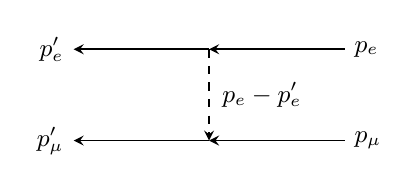
\begin{tikzpicture}[baseline=-.45ex,x=1cm,y=1cm,>=stealth,line width=.6pt,font=\small]
  \coordinate (tl) at (-1.72,.58);
  \coordinate (tc) at (0,.58);
  \coordinate (tr) at (1.72,.58);
  \coordinate (bl) at (-1.72,-.58);
  \coordinate (bc) at (0,-.58);
  \coordinate (br) at (1.72,-.58);
  \draw[<-] (tl)--(tc);
  \draw[<-] (tc)--(tr);
  \draw[<-] (bl)--(bc);
  \draw[<-] (bc)--(br);
  \draw[dashed,->] (tc)--(bc);
  \node[left] at (tl) {$p'_e$};
  \node[right] at (tr) {$p_e$};
  \node[left] at (bl) {$p'_\mu$};
  \node[right] at (br) {$p_\mu$};
  \node[right] at (.04,0) {$p_e-p'_e$};
\end{tikzpicture}
\tag{137.3}
\end{equation}
The corresponding amplitude is
\begin{equation}
M_{fi}^{(1)}=\frac{4\pi\alpha}{t}
(\bar u^{(\mu)'}\gamma^\nu u^{(\mu)})
(\bar u^{(e)'}\gamma_\nu u^{(e)}).
\tag{137.4}
\end{equation}
The limiting case (137.2) is obtained in this expression by replacing the matrix 4-vector $\gamma^\nu$ by its ``projection'' $\gamma^\nu_\perp$ onto the plane normal to the plane of $p_e$, $p'_e$ (or, equivalently, to the plane of $p_\mu$, $p'_\mu$, since in ultrarelativistic backward scattering $p_e\approx p'_\mu$, $p'_e\approx p_\mu$). Indeed, the matrix components parallel to the plane of $p_e$, $p'_e$ are
\[
\frac{1}{\sqrt{s}}(\gamma p_e+\gamma p'_e),\qquad
\frac{1}{\sqrt{s}}(\gamma p_e-\gamma p'_e)
\]
(the first is $\gamma^0$, while the second equals $\mathbf n_e\boldsymbol\gamma$, where $\mathbf n_e$ is the unit vector along $\mathbf p_e$). The Dirac equations for the bispinors $u^{(e)}$ and $u^{(\mu)}$ show that $(\bar u^{(\mu)'}\gamma^\nu u^{(\mu)})(\bar u^{(e)'}\gamma_\nu u^{(e)})\sim1/s$, so these terms may be omitted.

\SourcePage{680}{685}
At the next order one must add the diagram
\begin{equation}
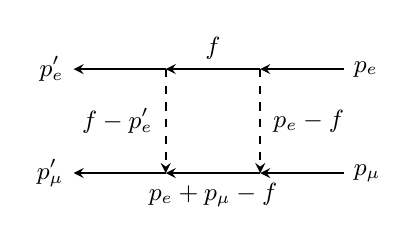
\begin{tikzpicture}[baseline=-.45ex,x=1cm,y=1cm,>=stealth,line width=.6pt,font=\small]
  \coordinate (tl) at (-1.65,.66);
  \coordinate (t1) at (-.48,.66);
  \coordinate (t2) at (.72,.66);
  \coordinate (tr) at (1.78,.66);
  \coordinate (bl) at (-1.65,-.66);
  \coordinate (b1) at (-.48,-.66);
  \coordinate (b2) at (.72,-.66);
  \coordinate (br) at (1.78,-.66);
  \draw[<-] (tl)--(t1); \draw[<-] (t1)--(t2); \draw[<-] (t2)--(tr);
  \draw[<-] (bl)--(b1); \draw[<-] (b1)--(b2); \draw[<-] (b2)--(br);
  \draw[dashed,->] (t1)--(b1);
  \draw[dashed,->] (t2)--(b2);
  \node[left] at (tl) {$p'_e$}; \node[right] at (tr) {$p_e$};
  \node[left] at (bl) {$p'_\mu$}; \node[right] at (br) {$p_\mu$};
  \node[above] at (.12,.66) {$f$};
  \node[left] at (-.52,0) {$f-p'_e$};
  \node[right] at (.76,0) {$p_e-f$};
  \node[below] at (.12,-.66) {$p_e+p_\mu-f$};
\end{tikzpicture}
\tag{137.5}
\end{equation}
and also the diagram with ``crossed'' photon lines. It is conveniently drawn in a form differing from (137.5) only in the direction of one solid line:
\begin{equation}
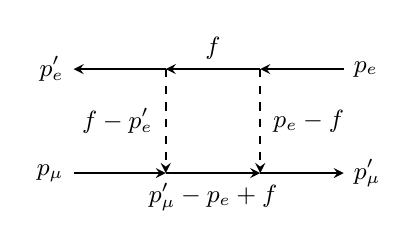
\begin{tikzpicture}[baseline=-.45ex,x=1cm,y=1cm,>=stealth,line width=.6pt,font=\small]
  \coordinate (tl) at (-1.65,.66);
  \coordinate (t1) at (-.48,.66);
  \coordinate (t2) at (.72,.66);
  \coordinate (tr) at (1.78,.66);
  \coordinate (bl) at (-1.65,-.66);
  \coordinate (b1) at (-.48,-.66);
  \coordinate (b2) at (.72,-.66);
  \coordinate (br) at (1.78,-.66);
  \draw[<-] (tl)--(t1); \draw[<-] (t1)--(t2); \draw[<-] (t2)--(tr);
  \draw[->] (bl)--(b1); \draw[->] (b1)--(b2); \draw[->] (b2)--(br);
  \draw[dashed,->] (t1)--(b1);
  \draw[dashed,->] (t2)--(b2);
  \node[left] at (tl) {$p'_e$}; \node[right] at (tr) {$p_e$};
  \node[left] at (bl) {$p_\mu$}; \node[right] at (br) {$p'_\mu$};
  \node[above] at (.12,.66) {$f$};
  \node[left] at (-.52,0) {$f-p'_e$};
  \node[right] at (.76,0) {$p_e-f$};
  \node[below] at (.12,-.66) {$p'_\mu-p_e+f$};
\end{tikzpicture}
\tag{137.6}
\end{equation}

Examination of the corresponding integrals shows that both diagrams acquire double-logarithmic contributions from regions of soft virtual photons: $|(f-p_e)^2|\ll m_e^2$ or $|(f-p'_e)^2|\ll m_e^2$. These contributions are associated with infrared divergences of the integrals and, by the argument above, must certainly cancel in the present case. Diagram (137.6), however, has a further double-logarithmic contribution from the region of large momenta: $|f^2|\gg m_\mu^2$. It is this contribution that must be evaluated.

The integral corresponding to diagram (137.6) is
\begin{equation}
M_{fi}^{(2)}=-i\frac{\alpha^2}{\pi^2}\int
\frac{(\bar u^{(e)'}\gamma^\nu(\gamma f+m_e)\gamma^\lambda u^{(e)})
(\bar u^{(\mu)'}\gamma^\lambda(\gamma f+m_\mu)\gamma_\nu u^{(\mu)})}
{(p'_e-f)^2(f^2-m_e^2)(f^2-m_\mu^2)(p_e-f)^2}\,d^4f,
\tag{137.7}
\end{equation}
where $p_e\approx p'_\mu$ has already been used. Put once more
\begin{equation}
f=up_e+vp'_e+f_\perp
\tag{137.8}
\end{equation}
(cf. (137.13)). The double-logarithmic contribution comes from the region specified by
\begin{equation}
|su|,\ |sv|\gg\rho\gg m_\mu^2;\qquad m_\mu^2/s\ll|u|,\ |v|\ll1,
\tag{137.9}
\end{equation}
where $\rho=-f_\perp^2$. In (137.8), the 4-vector $f_\perp$ is defined by $f_\perp p_e=f_\perp p'_e=0$; here (for backward scattering) it follows that $f_\perp^0=0$ in the centre-of-mass system, and hence $\rho=\mathbf f_\perp^2$.

In the numerator of the integral (137.7), $m_e$, $m_\mu$, and all terms containing $u$ or $v$ may be neglected; factors $u$ or $v$ in the numerator

\SourcePage{681}{686}
cancel the corresponding poles in the denominator (see below), preventing the required squared logarithms from arising. Noting that $(p'_e-f)^2\approx tu\approx-su$, $(p_e-f)^2\approx-sv$, $f^2\approx suv-\rho$, and transforming the integration element $d^4f$ according to (135.16), we rewrite (137.7) as
\[
M_{fi}^{(2)}=-i\frac{\alpha^2}{2\pi^2}\int
\frac{(\bar u^{(e)'}\gamma^\nu(\gamma f_\perp)\gamma^\lambda u^{(e)})
(\bar u^{(\mu)'}\gamma_\lambda(\gamma f_\perp)\gamma_\nu u^{(\mu)})}
{su\cdot sv(suv-\rho+i0)}\,s\,du\,dv\,d^2f_\perp.
\]
The numerator of the integrand is then transformed by averaging over the direction of $f_\perp$ and replacing $\gamma^\nu$, $\gamma^\lambda$ by $\gamma^\nu_\perp$, $\gamma^\lambda_\perp$ (for the same reasons as in (137.4)). Straightforward transformations give
\begin{equation}
M_{fi}^{(2)}=M_{fi}^{(1)}J^{(1)},\qquad
J^{(1)}=-i\frac{\alpha}{4\pi^2}\int
\frac{\rho\,du\,dv\,d\rho}{uv(suv-\rho+i0)^2}.
\tag{137.10}
\end{equation}
Finally, using the identity $\rho=(\rho-suv)+suv$ in the numerator, the second term may be dropped: it would cancel the simple poles and therefore yield no double-logarithmic contribution. Thus
\begin{equation}
J^{(1)}=-i\frac{\alpha}{4\pi^2}\int
\frac{du\,dv\,d\rho}{uv(\rho-suv-i0)}.
\tag{137.11}
\end{equation}

This integral has the same form as (135.20), and the integration over $\rho$ is consequently performed in the same way. Since now $\rho\gg m_\mu^2$, however, the condition becomes $suv\gg m_\mu^2$ (rather than $suv>0$). We then obtain
\begin{equation}
J^{(1)}=\frac{\alpha}{2\pi}\int\frac{du\,dv}{uv},
\tag{137.12}
\end{equation}
with the integration region bounded by
\[
m_\mu^2/s<u,\ v<1,\qquad suv>m_\mu^2
\]
(in a calculation to logarithmic accuracy, the strong inequalities $\gg$ are replaced by ordinary inequalities $>$). Direct evaluation gives
\begin{equation}
J^{(1)}=\frac{\alpha}{4\pi}\ln^2\frac{s}{m_\mu^2}.
\tag{137.13}
\end{equation}

At higher orders of perturbation theory, the contributions $\sim\alpha^n\ln^{2n}s$ of interest arise from ``ladder'' diagrams analogous to (137.6), with more ``rungs''. The full double-logarithmic asymptotic form

\SourcePage{682}{687}
of the scattering amplitude is therefore given by the infinite sum
\begin{equation}
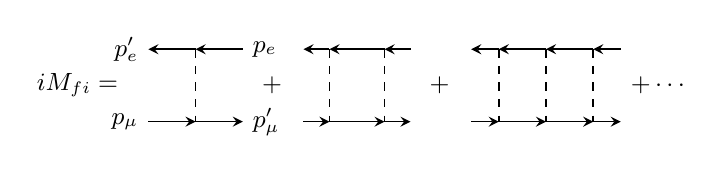
\begin{tikzpicture}[baseline=-.45ex,x=1cm,y=1cm,>=stealth,line width=.6pt,font=\small]
  \node at (-4.05,0) {$iM_{fi}=$};
  % one rung
  \draw[<-] (-3.15,.46)--(-2.55,.46); \draw[<-] (-2.55,.46)--(-1.95,.46);
  \draw[->] (-3.15,-.46)--(-2.55,-.46); \draw[->] (-2.55,-.46)--(-1.95,-.46);
  \draw[dashed] (-2.55,.46)--(-2.55,-.46);
  \node[left] at (-3.15,.46) {$p'_e$};
  \node[right] at (-1.95,.46) {$p_e$};
  \node[left] at (-3.15,-.46) {$p_\mu$};
  \node[right] at (-1.95,-.46) {$p'_\mu$};
  \node at (-1.58,0) {$+$};
  % two rungs
  \draw[<-] (-1.18,.46)--(-.85,.46); \draw[<-] (-.85,.46)--(-.15,.46); \draw[<-] (-.15,.46)--(.18,.46);
  \draw[->] (-1.18,-.46)--(-.85,-.46); \draw[->] (-.85,-.46)--(-.15,-.46); \draw[->] (-.15,-.46)--(.18,-.46);
  \draw[dashed] (-.85,.46)--(-.85,-.46);
  \draw[dashed] (-.15,.46)--(-.15,-.46);
  \node at (.55,0) {$+$};
  % three rungs
  \draw[<-] (.95,.46)--(1.30,.46); \draw[<-] (1.30,.46)--(1.90,.46); \draw[<-] (1.90,.46)--(2.50,.46); \draw[<-] (2.50,.46)--(2.85,.46);
  \draw[->] (.95,-.46)--(1.30,-.46); \draw[->] (1.30,-.46)--(1.90,-.46); \draw[->] (1.90,-.46)--(2.50,-.46); \draw[->] (2.50,-.46)--(2.85,-.46);
  \draw[dashed] (1.30,.46)--(1.30,-.46);
  \draw[dashed] (1.90,.46)--(1.90,-.46);
  \draw[dashed] (2.50,.46)--(2.50,-.46);
  \node[right] at (2.85,0) {$+\cdots$};
\end{tikzpicture}
\tag{137.14}
\end{equation}
To establish the general form of the terms in this sum, consider also the third-order diagram (the third term of the series (137.14)). Its integral may be reduced to
\begin{equation}
M_{fi}^{(3)}=M_{fi}^{(1)}J^{(2)},\qquad
J^{(2)}=\left(\frac{\alpha}{2\pi}\right)^2
\int\frac{du_1\,dv_1\,du_2\,dv_2}
{u_1v_1(u_1+u_2)(v_1+v_2)}
\tag{137.15}
\end{equation}
over the region
\[
m_\mu^2/s<u_{1,2},\ v_{1,2}<1,\qquad su_1v_1,\ su_2v_2>m_\mu^2.
\]
The double-logarithmic part of this integral can be isolated by imposing the further conditions
\begin{equation}
v_2\gg v_1,\qquad u_2\gg u_1.
\tag{137.16}
\end{equation}
Then
\[
J^{(2)}=\left(\frac{\alpha}{2\pi}\right)^2
\int\frac{du_1\,dv_1\,du_2\,dv_2}{u_1u_2v_1v_2}
=\left(\frac{\alpha}{2\pi}\right)^2
\int d\xi_1\,d\eta_1\,d\xi_2\,d\eta_2,
\]
where $\xi_i=\ln(su_i/m_\mu^2)$, $\eta_i=-\ln v_i$, while the integration region is defined by
\[
\xi_1>\eta_1;\qquad \xi_2>\eta_2;\qquad
\sigma>\xi_2,\ \eta_2>0;\qquad \sigma=\ln(s/m_\mu^2).
\]
Similarly, the $n$th term of the series may be written as $M_{fi}^{(n)}=M_{fi}^{(1)}J^{(n)}$, where
\begin{equation}
J^{(n)}(\sigma)=\left(\frac{\alpha}{2\pi}\right)^2
\int d\xi_1\,d\eta_1\ldots d\xi_n\,d\eta_n,
\tag{137.17}
\end{equation}
and the integration region is
\begin{equation}
\xi_i>\eta_i\quad(i=1,2,\ldots,n),\qquad
\sigma>\xi_n,\ \eta_n>0.
\tag{137.18}
\end{equation}
The complete scattering amplitude equals
\begin{equation}
M_{fi}=M_{fi}^{(1)}\left[1+\sum_{n=1}^{\infty}J^{(n)}(\sigma)\right].
\tag{137.19}
\end{equation}

To evaluate this sum, introduce auxiliary functions $A^{(n)}(\xi,\eta)$ given by the same integrals (137.17), but with the integration regions
\begin{equation}
\xi_i>\eta_i\quad(i=1,2,\ldots,n),\qquad
\xi>\xi_n>0,\qquad \eta>\eta_n>0
\tag{137.20}
\end{equation}

\SourcePage{683}{688}
(different upper limits for the integrations over $\xi_n$ and $\eta_n$, instead of the equal ones in (137.18)). Clearly $M_{fi}=M_{fi}^{(1)}A(\sigma,\sigma)$, where
\begin{equation}
A(\xi,\eta)=\sum_{n=0}^{\infty}A^{(n)}(\xi,\eta),\qquad A^{(0)}=1.
\tag{137.21}
\end{equation}

The definition of $A^{(n)}(\xi,\eta)$ shows that these functions obey the recurrence relations
\[
A^{(n)}(\xi,\eta)=\frac{\alpha}{2\pi}\int d\xi_1\,d\eta_1
A^{(n-1)}(\xi_1,\eta_1).
\]
Summing these relations over $n$ from 1 to $\infty$ gives the integral equation determining $A(\xi,\eta)$:
\begin{equation}
A(\xi,\eta)=1+\frac{\alpha}{2\pi}\int A(\xi_1,\eta_1)\,d\xi_1\,d\eta_1,
\tag{137.22}
\end{equation}
\[
\xi_1>\eta_1,\qquad \xi>\xi_1>0,\qquad \eta>\eta_1>0.
\]
For what follows it is enough to consider $A(\xi,\eta)$ in the region $\xi>\eta$. Equation (137.22) can then be written
\begin{equation}
A(\xi,\eta)=1+\frac{\alpha}{2\pi}
\int_0^\eta\!d\eta_1\int_{\eta_1}^\xi\!A(\xi_1,\eta_1)\,d\xi_1.
\tag{137.23}
\end{equation}
Differentiating this equality with respect to $\eta$ gives
\begin{equation}
\frac{\partial A(\xi,\eta)}{\partial\eta}
=\frac{\alpha}{2\pi}\int_\eta^\xi A(\xi_1,\eta)\,d\xi_1,
\tag{137.24}
\end{equation}
and a further differentiation with respect to $\xi$ yields the differential equation for $A(\xi,\eta)$,
\begin{equation}
\frac{\partial^2A}{\partial\eta\,\partial\xi}-\frac{\alpha}{2\pi}A=0.
\tag{137.25}
\end{equation}
This equation must be solved subject to the boundary conditions
\begin{equation}
A(\xi,0)=1,\qquad
\left.\frac{\partial A}{\partial\eta}\right|_{\xi=\eta}=0,
\tag{137.26}
\end{equation}
which follow directly from (137.23), (137.24).

The solution can be found by applying a Laplace transform in $\xi$:
\begin{equation}
A(\xi,\eta)=\frac{1}{2\pi i}\int_C e^{p\xi}Q(p,\eta)\,dp,
\tag{137.27}
\end{equation}

\SourcePage{684}{689}
where the contour $C$ in the complex $p$ plane is a closed curve enclosing $p=0$. Substitution of (137.27) into (137.25), followed by setting the integrand to zero, gives
\[
p\frac{\partial Q}{\partial\eta}=\frac{\alpha}{2\pi}Q,
\qquad Q=\varphi(p)\exp\frac{\alpha\eta}{2\pi p},
\]
where $\varphi(p)$ is arbitrary. The first boundary condition in (137.26) now gives $\varphi(p)=1/p+\psi(p)$, where $\psi(p)$ is analytic and has no singularities within $C$. The second condition in (137.26) is satisfied by choosing $\psi(p)=-2\pi p/\alpha$; indeed, then
\[
\left.\frac{\partial A}{\partial\eta}\right|_{\xi=\eta}
=-\frac{1}{2\pi i\xi}\int_C\frac{d}{dp}
\exp\xi\left(p+\frac{\alpha}{2\pi p}\right)dp=0.
\]

Collecting the results and setting $\xi=\eta=\sigma$, we find
\[
A(\sigma,\sigma)=-\frac{1}{2\pi i}\frac{2\pi}{\alpha\sigma}
\int_C p\frac{d}{dp}\exp\left[\sigma\left(p+\frac{\alpha}{2\pi p}\right)\right]dp.
\]

Finally, integrating by parts and using the known formula
\[
I_1(z)=\frac{1}{2\pi i}\int_C\exp\left[\frac z2\left(p+\frac1p\right)\right]dp
\]
($I_1(z)=-iJ_1(iz)$ is the Bessel function of imaginary argument), the scattering amplitude is ultimately
\begin{equation}
M_{fi}=M_{fi}^{(1)}\sqrt{\frac{2\pi}{\alpha\sigma^2}}
I_1\left(\sqrt{\frac{2\alpha}{\pi}}\,\sigma\right).
\tag{137.28}
\end{equation}
The scattering cross-section (for the angle $\theta=\pi$) is accordingly
\begin{equation}
d\sigma=d\sigma^{(1)}\frac{2\pi}{\alpha\ln^2(s/m_\mu^2)}
I_1^2\left(\sqrt{\frac{2\alpha}{\pi}}\ln\frac{s}{m_\mu^2}\right),
\qquad d\sigma^{(1)}=\frac{2\pi\alpha^2}{s^2}\,dt,
\tag{137.29}
\end{equation}
where $d\sigma^{(1)}$ is the Born-approximation cross-section in the ultrarelativistic case (see Problem 6, \S~81)\footnote{Further references to work on double-logarithmic asymptotics can be found in the review article: Gorshkov V.~G.//UFN.---1973.---Vol.~110.---P.~45.}.
